\documentclass[10pt]{article}

\usepackage[utf8]{inputenc}
\usepackage[portuguese]{babel}
\usepackage{auto-pst-pdf}
\usepackage{fullpage}
\usepackage{latexsym}
\usepackage{vaucanson-g}
\usepackage{amsmath}
\usepackage{amssymb}
\usepackage{amsthm}

\newcommand{\quest}[1] {\vspace{0.5cm}\noindent {\bf {#1})}\\}
\newcommand{\partQuest}[1] {\noindent {\bf {#1})}}
\newcommand{\fimprova}{\begin{flushright}$\Box$\end{flushright}}

\newtheorem{thm}{Theorem}[section]
\newtheorem{fact}[thm]{Fact}

%%%%%%%%%%%%%%%%%%%%%%%%%%%%%%%%%%%%%%%%%%%%%%%%%%%%%
%
%
%			Título
%
%
%%%%%%%%%%%%%%%%%%%%%%%%%%%%%%%%%%%%%%%%%%%%%%%%%%%%%
\title{ {\footnotesize
	\hrule\vspace{1pt}\hrule\vspace{1ex}
		Instituto de Computação \hfill Universidade Estadual de Campinas
	\smallskip 
	\hrule\vspace{1pt}\hrule}\vspace{10pt}
		MO405 --- Teoria de Grafos I \\[-6pt]
	\author{Jefferson e Rafael} 
}

\date{\bf Primeiro Semestre de 2011}

%%%%%%%%%%%%%%%%%%%%%%%%%%%%%%%%%%%%%%%%%%%%%%%%%%%%%
%
%
%			Soluçőes
%
%
%%%%%%%%%%%%%%%%%%%%%%%%%%%%%%%%%%%%%%%%%%%%%%%%%%%%%
\begin{document}
 
\maketitle
\vspace{0.5cm}
\thispagestyle{empty}


% Questőes
% ==================== PRIMEIRA LISTA =====================
%\quest{1.1.2}

Seja $G$ um grafo simples com $n$ vértices numerados de $1$ até $n$.
%
Considere a matriz de adjacências {\bf A}$_{n,n}$ associada a $G$.
%
Neste caso a matriz é definida como $${\bf A}_{i,j} = \left\{ \begin{array}{lr} 1, & se\quad\{i,j\} \in E(G) \\ 0, & c. c. \end{array}\right.$$
%
Como $G$ é simples $A_{i,i}$, $1 \le i \le n$ e, portanto, $\sum_{1 \le i \neq j \le n} A_{i_j} \le n\cdot (n-1)$.
%
Pelo teorema fundamental temos que 
\begin{eqnarray}
	2m &=& \sum_{1 \le i \neq j \le n} A_{i_j} \le n\cdot(n-1) \nonumber\\
	m  &\le& \frac{n\cdot(n-1)}{2} = \left(\begin{array}{c} n \\ 2 \end{array}\right) \nonumber
\end{eqnarray}
\fimprova

Além disto, quando $G$ é completo ($K_n$) temos que a matriz {\bf A} fica definida como $${\bf A}_{i,j} = \left\{ \begin{array}{lr} 1, & se\quad ssi\neq j \\ 0, & c. c. \end{array}\right.$$ logo
\begin{eqnarray}
	2m &=& \sum_{1 \le i \neq j \le n} A_{i_j} = n\cdot(n-1) \nonumber\\
	m  &=& \frac{n\cdot(n-1)}{2} = \left(\begin{array}{c} n \\ 2 \end{array}\right) \nonumber
\end{eqnarray}
\fimprova

%\quest{1.1.3}

\partQuest{a} Seja $G[X,Y]$ um grafo simples bipartido, onde $|X| = r$ e $|Y| = s$, considere a matriz de adjac�ncias {\bf A}$_{r,s}$ associada a $G$.
%
Neste caso a matriz � definida como $${\bf A}_{i,j} = \left\{ \begin{array}{lr} 1, & se\quad\{i,j\} \in E(G) \\ 0, & c. c. \end{array}\right.$$
%
Portanto, como n�o h� v�rtices repitidos nas linhas e colunas da matriz {\bf A} temos que $$m = \sum_{\substack{1 \le i \le r \\ 1 \le j \le s}} A_{ij} \le rs$$.
\fimprova

\partQuest{b} Basta mostrar o m�ximo da fun��o $f(r,s) = r.s$, onde $1 \le r \le n$, $1 \le s \le n$ e $r = s$.
%
Para isto buscamos os pontos cr�ticos de $f$ com: 
\begin{eqnarray}
	\frac{\partial f}{\partial r} = 0 &\Rightarrow& s = 0 \nonumber\\
	\frac{\partial f}{\partial s} = 0 &\Rightarrow& r = 0 \nonumber
\end{eqnarray}
Como nenhum dos pontos pertence ao dom�nio, devemos analisar os pontos extremais nos limites do dom�nio, em particular, quando $r = s$.
%
Neste caso, $f(r,s) = r(n - r) = nr - r^2$, onde $n$ � constante e $1 \le r \le n$.
%
Buscando os pontos de m�nimo temos: $$\frac{\partial f}{\partial r} = 0 \Rightarrow n - 2r = 0 \Rightarrow r = \frac{n}{2}$$

Al�m disto, � $n = \frac{r}{2}$ � ponto de m�ximo pois: $$\frac{\partial f^2}{\partial r\partial r} = -2 < 0$$.

Portanto, o m�ximo da fun��o $f$ ocorre quando $r = s = \frac{n}{2}$ com valor $\frac{n^2}{4}$.
\fimprova

\partQuest{b} Os grafos bipartidos completos $K_{\frac{n}{2},\frac{n}{2}}$ possuem $n$ v�rtices e, exatamente $\frac{n^2}{4}$ arestas.



% ==================== SEGUNDA LISTA ======================
\quest{4.1.1}

\partQuest{a} {\bf Sol 1)} Provaremos primeiro um resultado mais genérico.
%
Seja $F$ uma floresta com $\Delta(F) = k$, então $F$ tem pelo menos $k$ folhas (Denote por $\# folhas(G)$ o número de folhas na árvore $G$). A prova será por indução forte em $e(F)$.

Se $e(F) = 0$, então o resultado segue trivialmente pois $\# folhas(F) \ge 0$.
%
Caso contrário, seja $P = v_1v_2v_3\ldots v_k$ um caminho maximal em $F$ com $k \ge 2$ (Podemos escolher isto, já que $E(F) \ne \varnothing$).
%
Sabemos então, que $v_1$ e $v_k$ são folhas em $F$, senão ou $P$ não seria maximal ou haviria um ciclo em $F$.
%
Considere então $F' := (V(F),E(F)-E(P))$, que é uma floresta (não contém ciclos), com $e(F') < e(F)$, duas folhas a menos ($v_1$ e $v_k$) e $\Delta(F') \ge \Delta(F) - 2$, pois $\forall v\in V(F)\quad d_F(v) \ge d_{F'}(v) - 2$, já que removemos as arestas de um caminho.
%
Por hipótese de indução, temos que $\# folhas(F') \ge \Delta(F')$.
%
Logo, temos o seguinte: 
\begin{eqnarray}
	\#folhas(F) &=& \# folhas(F') + 2  \nonumber \\
		  &\ge& \Delta(F') + 2 	   \nonumber \\
		  &\ge& \Delta(F) - 2 + 2  \nonumber \\
		    &=& \Delta(F) \nonumber
\end{eqnarray}
\fimprova

Como corolário deste resultado temos a resposta da questão, para o caso em que $F$ é conexa.\\

\partQuest{b} Um conjunto ${\cal P} = \{P_1, P_2, \ldots, P_k\}$, onde $P_i$, $1 \le i \le k$, é um caminho. Além disto, os caminhos são disjuntos nos vértices, exceto pelo vertice inicial $x$, que é comum a todos.
%
Por exemplo ${\cal P} = \{ xv_1v_2v_3, xz_1z_2z_3z_4, xq_1q_2\}$, que pode ser visto na Figura \ref{graph:estrelaGrande}.
%
Neste caso, temos $d(x) = k$, $d(y) = 2$ (quando $y$ não está no final de algum caminho) e $d(s) = 1$ para os últimos vértices de cada caminho.
%
Além disto, temos $k$ folhas (uma de cada caminho).
%%%%%%%%%%%%%%%%%%%%%%%%%%%%%%%%%%%%%%%%%%%%%%%%%%%%%
%
%
%                       Delta(G) = #folhas(G)
%
%
%%%%%%%%%%%%%%%%%%%%%%%%%%%%%%%%%%%%%%%%%%%%%%%%%%%%%
\begin{figure} [htb]
        \centering
        \begin{postscript}
                \TinyPicture\VCDraw{%
                \begin{VCPicture}{(0,0)(12,12)}
                        \ChgEdgeArrowStyle{-}
                        %%%%%%%%%%%%%%%%%%%%%%%%%%%% vertices %%%%%%%%%%%%%%%%%%%%%%%%%
                        % Vértice em comum
                        \State[x]{(6,6)}{1}
			% Caminho v
			\State[v_1]{(8,6)}{2} \State[v_2]{(10,6)}{3} \State[v_3]{(12,6)}{4}
                        % Caminho q
                        \State[q_1]{(4,4)}{5} \State[q_2]{(2,2)}{6}
			% Caminho z
			\State[z_1]{(4,8)}{7} \State[z_2]{(2,10)}{8} \State[z_3]{(0,12)}{9}
                        %%%%%%%%%%%%%%%%%%%%%%%%%%%% Arestas %%%%%%%%%%%%%%%%%%%%%%%%%
			% caminho v
                        \EdgeL{1}{2}{} \EdgeL{2}{3}{} \EdgeL{3}{4}{}
			% caminho q
                        \EdgeL{1}{5}{} \EdgeL{5}{6}{}
			% caminho z
                        \EdgeL{1}{7}{} \EdgeR{7}{8}{} \EdgeL{8}{9}{}
                \end{VCPicture}}
        \end{postscript}
        \caption {Grafo $G$ com $\Delta(G) = \#folhas(G)$.}
	\label{graph:estrelaGrande}
\end{figure}



\quest{4.1.2}

Vamos provar que a) $\leftrightarrow$ c) e b) $\leftrightarrow$ c).

\partQuest{a}

\partQuest{b}
($\Rightarrow$) Seja $G$ uma floresta com $n-1$ arestas.
%
Como florestas são acíclicas, basta mostrar que $c(G) = 1$ e teremos então uma árvore. 
%
Considere então ${\cal C} = \{c_1, c_2, \ldots, c_k\}$ as componentes conexas de $G$.
%
Cada componente $c_i$ é um grafo conexo, acíclico e com $e(C_i) = v(c_i) - 1$, pois é uma árvore ({\bf Teorema 4.3}).
%
Desta forma, a quantidade de arestas em $G$ é dada por:
\begin{eqnarray}
	e(G) &=& \sum_{c_i \in {\cal C}} e(c_i)      \nonumber \\
	     &=& \sum_{c_i \in {\cal C}} v(c_i) - 1  \nonumber \\
	     &=& \sum_{c_i \in {\cal C}} v(c_i) - \sum_{c_i \in {\cal C}} 1 \nonumber \\
	     &=& n - k \label{eq:componentes}
\end{eqnarray}

Logo, como temos $n-1$ arestas em $G$, então $k = 1$, com o conjunto $|{\cal C}| = 1$ e, portanto, $G$ uma árvore.

($\Leftarrow$) Seja $G$ uma árvore, então, por definição $G$ é floresta. Além disto, $c(G) = 1$ e, utilizando a equação \ref{eq:componentes}, temos que $e(G) = n - 1$ e o resultado segue.
\fimprova


\quest{4.1.4}
Sejam $G$ e $F$ como na hipótese. Porque $F$ é uma floresta maximal, $F$ induz
uma subárvore geradora em cada componente de $G$. Sejam $C_1,C_2,\cdots,C_{c(G)}$
as componentes de $G$ e $F_1,F_2,\cdots,F_{c(G)}$ as subárvores geradoras de cada
componente. Para cada $F_i$, vale $e(F_i) = v(C_i) - 1$, $1 \le i \le c(G)$.
Somando para todo $F_i$ temos que
\[
    e(F) = \sum^{c(G)}_{i=1} e(F_i) = \sum^{c(G)}_{i=1} (v(C_i) - 1) = \sum^{c(G)}_{i=1} v(C_i) - c(G) = v(G) - c(G).
\]
\fimprova


\quest{4.1.6}

Seja $x \in V(D)$ e $X=\{v: v \in v(D)$ e $\exists xDv\}$.
%
Considere então o subgrafo induzido $D'$ pelos vértices em $X$ ($D' := D[X]$).
%
Remova todos os arcos com cabeça em $x$, pois queremos um $x$-{\it branching}.
%
Todos os vértices ainda permanecem alcançáveis, pois estes arcos não estavam em nenhum caminho orientado entre $x$ e $v$, $v \in V(D')$ (estavam em passeios orientados).
%
Se $\forall v \in V(D')\quad d^-(v) = 1$, então já temos um $x$-{\it branching}.
%
Caso contrário, seja $v \in V(D')$, onde $d^-(v) > 1$, então remova um dos arcos com cabeça em $v$.
%
Neste caso, $v$ ainda será alcançável a partir de $x$, pois ainda há um caminho $xD'v$ utilizando um dos arcos $(v',v)$ restantes, pois $\exists xD'v'$.
%
Desta forma, remover um arco de vértices $v$, onde $d^-(v) > 1$, preserva a existência de caminho entre $x$ e $v$.
%
Portanto, repetindo este processo, eventualmente obteremos um $x$-{\it branching}, já que $e(D')$ é finito.
\fimprova

\quest{4.1.8}

\partQuest{a} Sejam $T$ e $T'$ como na hipótese, $D(v) = \max\{d(v,u) \, : u \in V\}$
tal que $D(v)$ é mínimo e $C = \{v_1, v_2, \cdots, v_k\}$ os centros de $T$.

\begin{fact}
\label{fact:folhadist}
Se $D(v) = d(v, f)$ então $f$ é folha.
\end{fact}

\begin{proof} Suponha por absurdo $D(v)$ como na hipótese mas que $f$ não seja
folha. Porque $f$ não é folha, $f$ possui um vizinho $u \ne v$. Nesse caso,
$D'(v) = d(v, f) + 1 > D(v)$, o que é um absurdo.
\end{proof}

\begin{fact}
\label{fact:contained}
Em $T'$, $D_{T'}(u) = D_T(u) - 1$, $\forall u \in V(T')$.
\end{fact}

\begin{proof} Direta do Fato \ref{fact:folhadist} e da forma como $T'$ é obtida.
\end{proof}

Seja $C' = \{v'_1, v'_2, \cdots, v'_l\}$ os centros de $T'$. Do Fato
\ref{fact:contained}, obtemos que $C \subseteq C'$. Suponha agora por absurdo que
$\exists v'_i \in C' \setminus C$ tal que $D_{T'}(v'_i) \le D_{T'}(v)$, $v \in C$.
Então sabemos do Fato \ref{fact:contained} que
\begin{equation}
\label{eq:part1}
D_{T'}(v'_i) \le D_{T'}(v) = D_T(v) - 1
\end{equation}

Além do mais, sabemos que
\begin{equation}
\label{eq:part2}
D_{T'}(v'_i) \le D_T(v'_i) \le D_{T'}(v'_i) + 1
\end{equation}

Finalmente, temos de \eqref{eq:part1} e \eqref{eq:part2} que
\[D_T(v'_i) = D_{T'}(v'_i) + 1 \le D_T(v),\] o que é um absurdo pois nesse caso
$v'_i$ seria centro em $T$.

\partQuest{b}


\quest{4.1.20}

\partQuest{a}
($\rightarrow$) Suponha por absurdo que $T_1 \cap T_2 = \emptyset$. Se
$u \in V(T_1)$ e $v \in V(T_2)$ então não existe caminho de $u$ para $v$ em
$T_1 \cup T_2$. Mas isso contraria a hipótese de que $T_1 \cup T_2$ é uma
subárvore de $T$.

\partQuest{b}
Prova por indução forte em $|T_f| = n$.

Hipótese: Se $T_f$ é uma família de subárvores de uma árvore $T$ com $|T_f| = k$,
$ 1 \le k \le n$, se quaisquer 2 membros de $T_f$ possuem um vértice em comum,
então há um vértice de $T$ que pertence a todos os membros de $T_f$.

Passo: Seja $T_f$ uma família de subárvores da árvore $T$ como na hipótese e tal
que $|T_f| = n + 1$. Sejam $T'$ e $T''$ subárvores de $T_f$ tal que
$T' \cap T'' \ne \emptyset$. Sabemos de (a) que $T' \cap T''$ é subárvore de $T$.
Seja $T'_f = T_f - \{T', T''\} \cup \{T' \cap T''\}$ a família obtida por
substituir $T'$ e $T''$ por sua intersecção em $T_f$. Em $T'$, temos que
$T_i \cap T_j \ne \emptyset$, $\forall T_i, T_j$. Então, por H.I. existe um
vértice $v$ de $T$ que pertence a todos os membros de $T'_f$. Em particular, $v$
pertence a $T' \cap T''$ e, portanto, pertence a $T'$ e $T''$.
\fimprova

\quest{4.2.1}

\partQuest{a}


\partQuest{b} Seja $G$ um grafo conexo qualquer e $e = vx \in E(G)$, temos que para cada subárvore geradora $T$ de $G$, ou $e \in E(T)$ ou $e \notin E(T)$.
%
Se $e \notin E(T)$, então $T$ é arvore geradora de $G\backslash e$, caso contrário, se $e \in E(T)$, então pela letra (a) temos que $T/e$ é árvore geradora de $G/e$.
%
Logo, $$t(G) = t(G\backslash e) + t(G/e)$$

\quest{4.2.3}
\partQuest{a}
Vou mostrar como construir a {\it distance Tree} $T$ e depois demonstrarei que $\forall v \in V(G)\quad d_T(x,v) = d_G(x,v)$

Considere inicialmente $T:=({x},\varnothing)$, uma árvore que será aumentada a cada passo do processo. Seja  $V' = \{v: v \in V(G) - V(T)$ e $uv \in \partial(V(T))\}$.
%
Faça $T' := (V(T)\cup V', E(T)\cup E')$,  onde $E' \subseteq \partial(V(T))$ é o conjunto das arestas com extremos não repetidos em $V(G) - V(T)$ (Se $k$ arestas tem o mesmo extremo em $V(G) - V(T)$, escolha qualquer uma delas para fazer parte de $E'$).
%
Então, repita o processo com $T'$ enquanto $V(T') \ne V(G)$.

A cada passo inserimos, pelo menos, um vértice e uma aresta em $T$, pois $\partial(V) \ne \varnothing$ para todo $V \subset V(G)$ pois $V$ é conexo.
%
Portanto, eventualmente, o processo alcança $V(T) = V(G)$, logo o subgrafo $T$ de $G$ é gerador e, além disto, é uma árvore pois é conexo (pela forma como foi construído) e acíclico, pois as arestas inseridas em $T$ não geram ciclos, pois criam o primeiro e único caminho entre $u$ e $x$, onde $u \in V(T)$ e $v \in V(G)-V(T)$.

Mostrarei agora que $\forall v \in V(G)\quad d_T(x,v) = d_G(x,v)$. A prova será por indução fraca em $d_G(x,v)$.
%
Na base, considere que $d_G(x,v) = 1$, logo, pela forma com que $T$ é construída, temos que na primeira iteração do processo $T=({x},\varnothing)$, e $v\in V'$ pois ${x,v} \in \partial(\{x\})$.
%
Logo, pelo menos uma aresta incidente em $v$ será adicionada a $T$ e, portanto $d_T(x,v) = 1$.
%
Como Hipótese de Indução, tenho que se $d_G(x,v) = k$ então $d_T(x,v)$.
%
No passo, considere $v' \in V(G)$, onde, $d_G(x,v') = k + 1$.
%
Seja então $P_i = xv_{1i}v_{2i}\ldots v_{ji}v'$ caminhos de $x$ a $v'$ em $G$ com comprimento $k + 1$. 
%
Sabemos que $d_G(x,v_{ji}) = k$ $\forall i$, senão haveria um caminho menor que todos os caminhos $P_i$ de $x$ a $v'$.
%
Logo, por Hipótese de Indução, temos que $d_T(x,v_{ji}) = k$ e portanto, uma das arestas ${v_{ji},v'}$ será adicionada a $T$ em algum passo do processo descrito acima.
%
Portanto, $d_T(x,v') = d_T(x,v_{ji}) + 1 = k + 1$.
\fimprova

\partQuest{b}


\quest{4.2.8}

($\Leftarrow$) Sabemos que um digrafo é bipartido se e somente se todas suas
componentes fortes são bipartidas. Portanto se $D$ é um digrafo que contém uma
componente forte não bipartida, então $D$ não é bipartido. Pelo Teorema 4.7, $D$
não contém um ciclo ímpar. Isso significa que nenhuma das componentes fortes de
$D$ possui um ciclo impar. Portanto, pelo Exercício 3.4.11b, $D$ não possui ciclo
ímpar orientado.

($\Rightarrow$) Se um digrafo $D$ contém um ciclo orientado ímpar é porque alguma
de suas componentes fortes contém um ciclo orientado ímpar. Então, pelo Exercício
3.4.11b, $D$ possui um ciclo ímpar e do Teorema 4.7, $D$ não é bipartido. Mas se
$D$ não é bipartido então existe uma componente forte de $D$ tal que esta não é
bipartida.


\quest{4.2.9}

\partQuest{a}
($\Leftarrow$) Primeiramente vou mostrar como construir o {\it spanning x-branching} $S$ de $D$ para o $x \in V(D)$ como dado na hipótese.
%
Considere inicialmente $S := (\{x\}, \varnothing)$.
%
Enquanto $V(D)-V(S) \ne \varnothing$ repita o seguinte procedimento.
%
Como $V(D)-V(S) \ne \varnothing$, então existe, no mínimo, um arco $(v,v')$, onde $v \in V(D)$ e $v' \in V(S)$, pois $\partial^+(S) \ne \varnothing$.
%
Seja $V' = \{v: (u,v) \in \partial^+(S)$ e $E' \subseteq \partial^+(S)$ um subconjunto com apenas um arco incidindo em cada vértice (se mais de um arco incide em $z \in V(D)-V(S)$, remova uma delas).
%
Atualize $S := (V(S)\cup V', A(S) \cup E')$.

Basta-nos demonstrar que $S$ gerado é um {\it spanning x-branching}.
%
É gerador pois, a cada iteração incorpora, no mínimo, um vértice $v \in V(D)-V(S)$ e $V(D)$ é finito.
%
É {\it x-branching} pois $d^-(v) = 0$, pois $v$ nunca é adicionado novamente ao grafo $S$, logo $\nexists (.,x) \in A(S)$.
%
Além disto, $d^-(v) = 1$, $v\ne x$, pois a partir do momento em que um vértice $v$ é adicionado ao conjunto $V(S)$, ele nunca mais o será, pois não pertencerá a $V(D)-V(S)$.

($\Rightarrow$) Seja $S$ um {\it spanning x-branching} de $D$.
%
Seja $X \subset V(D)$, onde $x \in X$. Como $S$ é {\it spanning x-branching}, temos que $d^-(v) = 1$, $\forall v \in V(D)-X$ e, por definição, não há ciclos em $S$.
%
Logo, seja $P = v_1v_2\ldots v_k$ um caminho maximal em $V(D) - X$. Sabemos que $d^-(v_1) = 1$ e este arco incidente não pode ter cauda em $V(D) - X$ senão $P$ não seria maximal, ou existiria um ciclo em $S$ e em ambos os casos teríamos um absurdo.
%
Logo, $\exists (v',v_1) \in A(S)$, onde $v' \in X$, logo $|\partial^+(X)| \ge 1$, e, portanto, $\partial^+(X) \ne \varnothing$.
\fimprova

\partQuest{b} ($\Leftarrow$) Seja $D$ um digrafo para o qual existe um {\it spanning v-branching} $\forall v \in V(D)$.
%
Considere $x,y \in V(D)$, então num {\it spanning x-branching} existe um caminho orientado de $x$ para $y$, analogamente, num {\it spanning y-branching} há um caminho orientado de $y$ para $x$.
%
Desta forma, $D$ é fortemente conexo.

($\Rightarrow$) Seja $D$ um digrafo fortemente conexo.
%
Seja $x \in V(D)$ um vértice qualquer, temos que $\forall X \subset V(D)$, onde $x \in X$, existe um caminho de $x$ para $y \in V(D) - X$. Logo, $\partial^+(X) \ne \varnothing$ e, portanto, pela letra {\bf a)} temos que existe um {\it spanning x-branching} em $D$.


\quest{4.3.2}

\partQuest{a}
Seja $G$ um grafo qualquer e $T_1$ e $T_2$ duas subárvores geradoras de $G$.
%
Seja $e = xy \in T_1\backslash T_2$, considere então $T_1 - e$, e sabemos que como $e$ é uma aresta de corte, geraremos duas componentes conexas $X$ e $Y$, com os vértices alcancáveis a partir de $x$ e $y$, respectivamente (Veja a Figura \ref{graph:componentesT1-e}).
%
Como $e \notin T_2$, então $T_2 + e$ contém um ciclo fundamental e, portanto, existe uma aresta $f$ que liga algum $x' \in X$ a um $y' \in Y$.

Basta então mostrar que $T_1' := \{T_1 - e\} + f$, é acíclico e conexo.
%
Primeiramente, $T_1'$ é conexo pois existe caminho entre qualquer parte de vértices, $v$ e $v'$, internos em $X$ e $Y$ e, além disto, se $v$ e $v'$ estiverem em conjuntos diferentes ($v \in X$ e $v' \in Y$, sem perda de generalidade), então $\exists vXx'y'Yv'$ um caminho em $T_1'$.
%
Alem disto, $T_1'$ é acíclico, pois $T_1 - e$ o é, e se $f$ gerasse um ciclo em $T_1 - e$, então $\exists x'{T_1 - e}y'$ que não usa $f$, o que é uma contradição pois $x' \in X$ e $y' \in Y$ duas componentes conexas distintas em $T_1 - e$.
%%%%%%%%%%%%%%%%%%%%%%%%%%%%%%%%%%%%%%%%%%%%%%%%%%%%%
%
%
%                       Delta(G) = #folhas(G)
%
%
%%%%%%%%%%%%%%%%%%%%%%%%%%%%%%%%%%%%%%%%%%%%%%%%%%%%%
\begin{figure} [htb]
        \centering
        \begin{postscript}
                \TinyPicture\VCDraw{%
                \begin{VCPicture}{(0,0)(12,12)}
                        \ChgEdgeArrowStyle{-}
			%%%%%%%%%%%%%%%%%%%%%%%%%%%% Componentes %%%%%%%%%%%%%%%%%%%%%
			\FixStateDiameter{6cm} \ChgStateLabelScale{3} 
			\StateVar[X]{(2,6)}{X} \State[Y]{(10,6)}{X}  
			\LargeState \RstStateLabelScale 
                        %%%%%%%%%%%%%%%%%%%%%%%%%%%% vertices %%%%%%%%%%%%%%%%%%%%%%%%%
                        % Vértices de X
                        \State[x']{(4,4)}{1} \State[x]{(4,8)}{2}
                        % Vértices de y
                        \State[y']{(8,4)}{3} \State[y]{(8,8)}{4}
                        %%%%%%%%%%%%%%%%%%%%%%%%%%%% Arestas %%%%%%%%%%%%%%%%%%%%%%%%%
                        % arestas e e f
                        \ArcR{1}{3}{f} 
			\ChgEdgeLineStyle{dashed}
			\ArcL{2}{4}{e}
                \end{VCPicture}}
        \end{postscript}
        \caption {O grafo $T_1 - e$ e as arestas $e$ e $f$.}
        \label{graph:}
\end{figure}
\fimprova

\partQuest{b} É exatamente a questão anterior, invertendo $f$ por $e$.
\fimprova


\quest{4.3.3}
(a) $\Leftrightarrow$ (b) Se $S$ é árvore geradora, pela definição de que árvore
é um grafo acíclico conexo, $S$ não contém ciclos. Para ver que $S$ é maximal com
respeito a não ter ciclos, sejam $u,v \in V$ vértices não adjacentes em $S$. Como
$S$ é conexo, existe um caminho $uSv$ de $u$ para $v$ em $S$. Ao adicionar a aresta
$uv \in E$ a $S$ obtemos o ciclo $C:= uSvu$. Portanto, não existe árvore geradora
$S'$ com mais arestas que $S$ e que contenha $S$. Em contrapartida, se $S$ não
contém ciclos e é maximal, então $S$ é conexo, pois se existem dois vértices $u$
e $v$ entre os quais não há um caminho em $S$, adicionar a aresta $uv \in E$ gera
$S'$ acíclico com mais arestas que $S$, o que é absurdo.

(a) $\Leftrightarrow$ (c) Porque $S$ é conexa e geradora, todo corte de arestas
não vazio de $G$ contém pelo menos uma aresta de $S$. Se removermos uma aresta
qualquer, $S$ será disconexa e não encontrará o \emph{bond} de $G$ que contém a
aresta removida. Reciprocamente, se $S$ encontra todo \emph{bond} de $G$, então
$S$ é conexo e como é minimal com respeito a essa propriedade, $S$ não contém
ciclos. Portanto, $S$ é árvore geradora.


\quest{4.3.10}

\partQuest{a} Seja $G$ um grafo qualquer e $T_1$ e $T_2$ árvores geradoras de $G$ disjuntas. Vamos construir uma família de ciclos para depois utilizarmos o corolário {\bf 2.16} e mostrar que existe um subgrafo gerador par de $G$, logo, euleriano.

Considere $\overline{T_1}$, a {\it cotree} de $T_1$.
%
Seja ${\cal C} = \{c_e:$ um ciclo fundamental com $e \in \overline{T_1}\}$ uma família de cíclos.
%
Note que como $T_2 \subseteq \overline{T_1}$, então $\forall v \in V(G)\quad \exists c_e \in {\cal C}$, tal que $v \in c_e$, em especial quando $e = vx$, para algum $x \in V(G)$.

Portanto, o grafo $H_1 = \bigtriangleup {\cal C}$ é gerador e, pelo corolário {\bf 2.16}, é também um grafo par.
%
Logo, pelo Teorema {\bf 3.5} $G$ é euleriano.
\fimprova

\partQuest{b} Considere o grafo $H_1$ como gerado na letra {\bf a)} e, de forma semelhante, o grafo $H_2$ baseado em $T_2$ e $\overline{T_2}$.
%
Pelo que foi demonstrado em {\bf a)} temos que $H_1$ e $H_2$ são subgrafos pares geradores de $G$.%
Além disto, pelo Teorema {\bf 4.10} temos que $H_i \cap \overline{T_i} = \overline{T_i}$, $i = 1,2$, logo $\overline{T_i} \in H_i$.
%
Note também que $T_2 \subseteq \overline{T_1}$ e $T_1 \subseteq \overline{T_2}$, portanto: 
\begin{eqnarray}
	H_1 \cap H_2 &=& \overline{T_1} \cup \{H_1 - \overline{T_1}\} \cup \overline{T_2} \cup \{H_2 - \overline{T_2}\} \nonumber \\
		     &=& G \nonumber
\end{eqnarray}
\fimprova

\quest{5.1.1}

Primeiramente, podemos assumir que $G$ não tem loops, pois a remoção destes 
preserva o caminho entre qualquer par de vértices $v,v' \in V(G)$. Então seja 
$P = v_1,\ldots ,v_k$ um caminho maximal em $G$. Se $d(v_i) = 1$, $i \in \{1,k\}$, 
então este não é vértice de corte, pois não é vértice interno a nennhum caminho 
em $G$, e portanto sua remoção não aumenta o número de componentes de $G$. 
Caso contrário, temos que ou $d(v_1) > 1$ ou $d(v_k) > 1$ e, como assumimos que
$G$ não possui loops, sabemos que há arestas saindo de $v_1$ ou $v_k$ para
vértices de $P$. Para $v_1$, seja $v_i$, onde $\{v_1,v_i\} \in E(G)$, $G - v_1$
ainda possui caminhos entre todos os vértices, pois se $P' = xGv'v_1v''Gy$ era um 
caminho que ligava $x$ a $y$ em $G$, então $P'' = xGv'Pv''y$, pois $v_1$ está 
em um ciclo em $G$. O mesmo vale para $v_k$, invertendo os rótulos apenas.
Portanto $v_1$ e $v_k$ são vértices de corte em um grafo não trivial.
\fimprova


\quest{5.1.2}

Suponha por absurdo que $e = uv$ seja uma aresta de corte mas que nem $u$ nem
$v$ sejam vértices de corte de $G$. Isso significa que a remoção de $u$ ou $v$
não desconecta o grafo, o que implica que a remoção de $e$ também não
desconecta $G$, pois $G$ possui pelo menos 3 vértices. Mas isso contraria a
hipótese de que $e$ é aresta de corte.


\quest{5.1.3}

Para mostrar que $H$ não possui vértices de corte, basta mostrar que há dois
caminhos disjuntos entre qualquer par de seus vértices. Como isto já é válido
em $G$ e a inclusão de um vértice $v$ não altera isso, temos que basta provar
que $\exists P, P'$, onde $vPx,vP'x \in H$, $\forall x \in V(G)$ e que, além
disso $P \cap P' = \varnothing$.

%%%%%%%%%%%%%%%%%%%%%%%%%%%%%%%%%%%%%%%%%%%%%%%%%%%%%
%
%
%                       Delta(G) = #folhas(G)
%
%
%%%%%%%%%%%%%%%%%%%%%%%%%%%%%%%%%%%%%%%%%%%%%%%%%%%%%
\begin{figure} [htb]
        \centering
        \begin{postscript}
                \TinyPicture\VCDraw{%
                \begin{VCPicture}{(0,0)(12,12)}
                        \ChgEdgeArrowStyle{-}
			%%%%%%%%%%%%%%%%%%%%%%%%%%%% Componentes %%%%%%%%%%%%%%%%%%%%%
			\FixStateDiameter{7cm} \ChgStateLabelScale{3} 
			\StateVar[G]{(2,6)}{G}
			\LargeState \RstStateLabelScale 
                        %%%%%%%%%%%%%%%%%%%%%%%%%%%% vertices %%%%%%%%%%%%%%%%%%%%%%%%%
                        % Vértice v
                        \State[v]{(8,6)}{1}
			\State[a]{(4,7.5)}{2}
			\State[b]{(4,4.5)}{3}
                        %%%%%%%%%%%%%%%%%%%%%%%%%%%% Arestas %%%%%%%%%%%%%%%%%%%%%%%%%
                        % arestas e e f
                        \ArcR{1}{2}{e} 
			\ArcL{1}{3}{e'}
                \end{VCPicture}}
        \end{postscript}
        \caption {O grafo $H$.}
        \label{graph:HGe}
\end{figure}
\fimprova

Seja $x \in V(G)$, denote por $P$ e $P'$ dois caminhos disjuntos de $a$ a $x$ 
e ,$C$ e $C'$, dois caminhos disjuntos de $x$ a $b$. Seja $z$ o primeiro vértice
de $\{P \cup P'\} \cap C$. Sem perdade de generalidade $z \in P$, logo $vaPzCx$ é um
caminho entre $v$ e $x$, disjunto de $vbC'x$, devido a forma de escolha de $z$,
que garante que $bC' \cap aPzCx = \varnothing$.
\fimprova


\quest{5.1.4}

Se $X \cap Y \ne \varnothing$, todo vértice $v \in X \cap Y$ é um $(X,Y)$-path
de tamanho $0$ em $G$. Portanto, se $|X \cap Y| \ge 2$, o resultado segue. Se
$X \cap Y = \{v\}$, sabemos que $\exists x \in X$ e $\exists y \in Y$ e que,
porque $G$ não possui vértice de corte, existe um caminho $P$ que não passa por
$v$ entre $x$ e $y$. Se $x'$ é o último vértice de $X$ em $P$ e $y'$ o
primeiro, os caminhos $v$ e $x'Py'$ são $(X,Y)$-paths em $G$.

Suponha agora $X \cap Y = \varnothing$. Sejam $x, x' \in X$, $x \ne x'$, e
$y, y' \in Y$, $y \ne y'$, e $P_1, P_2$ e $P'_1, P'_2$ os caminhos internamente
disjuntos entre $x$ e $y$ e $x'$ e $y'$, respectivamente. Mostraremos como
construir dois caminhos disjuntos entre $X$ e $Y$. Seja $s \not \in X \cup Y$ o
primeiro vértice no qual os caminhos $P_1$ e $P'_1$ se interceptam. Considere o
caminho $P^1 = xP_1sP'_1y$ e seja $P = x''P_1sP'_1y''$ o caminho tal que $x''$
é o último vértice de $X$ em $P_1$ e $y''$ o primeiro em $Y$. Do mesmo modo,
seja $P' = x'''P'_2y'''$ o caminho tal que $x'''$ é o último vértice de $X$ em
$P'_2$ e $y'''$ o primeiro. Então, $P$ e $P'$ são dois $(X,Y)$-paths disjuntos.


\quest{5.1.5}

Seja $G$ um grafo conexo sem \emph{loop} e sem vértices de corte e sejam $C$
e $C'$ dois ciclos mais longos em $G$ com $|C| = |C'| = l$.

\begin{description}

\item[Caso 1.] Suponha por absurdo que $C$ e $C'$ tenham um vértice $x$ em
comum. Sejam $u$ e $v$ vértices de $G$ tais que $u \in C$, $v \in C'$ e $u,v
\ne x$. Porque $G$ não possui vértices de corte, existem dois caminhos
internamente disjuntos entre eles em $G$. Seja $P_{uv}$ um desses caminhos que
não passa por $x$. Em $P_{uv}$, considere os vértices $u_i$ e $v_j$, $u_i \in
C$ e $v_j \in C'$, tal que $u_i$ é o último vértice de $C$ em $P_{uv}$ e $v_j$
é o primeiro de $C'$ em $P_{uv}$ e seja $P = u_iP_{uv}v_j$ o subcaminho de
$P_{uv}$ entre eles (veja Figura~\ref{fig:ciclos}). Além do mais, sejam $P_1$ o
caminho vermelho entre $u_i$ e $v_j$ passando por $x$ e $P_2$ o caminho azul.

\begin{figure}[htb]
    \centering
    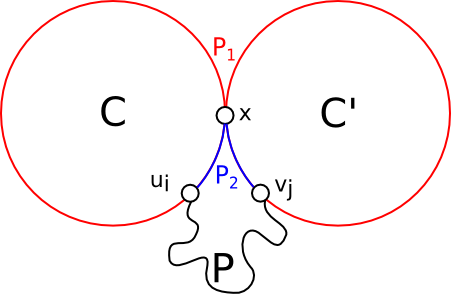
\includegraphics[height=5cm, width=7.67cm]{figuras/graph_q515}
    \caption{Ciclos mais longos em $G$}
    \label{fig:ciclos}
\end{figure}

    \begin{description}
        \item[Caso 1.1.] Se $i + j < l + 4$:

        então existe ciclo $C'' = P_1 \cup P$ tal que
        \begin{eqnarray}
            |C''| &=& l - i + 2 + l - j + 1 + |P| \nonumber \\
                &\ge& 2l - (i + j) + 4 \nonumber \\
                &>& 2l - (l + 4) + 4 = l \nonumber
        \end{eqnarray}
        é um ciclo mais longo que $C$ e $C'$ em $G$.

        \item[Caso 1.2.] Se não, se $i + j \ge l + 4$:

        então existe ciclo $C'' = P_2 \cup P$ tal que
        \begin{eqnarray}
            |C''| &=& i + j - 1 + |P| \nonumber \\
                 &\ge& i + j > l \nonumber
        \end{eqnarray}
        é um ciclo mais longo que $C$ e $C'$ em $G$.
    \end{description}

\item[Caso 2.] Suponha por absurdo que $C$ e $C'$ não tenham nenhum vértice em
comum. Sejam $s$ e $t$ vértices de $G$ tais que $s \in C$ e $t \in C'$. Porque
$G$ não possui vértices de corte, existem dois caminhos internamente disjuntos
entre eles em $G$. Seja $P_{st}$ um desses caminhos e sejam $s'$ o último
vértice de $C$ em $P_{st}$ e $t'$ o primeiro de $C'$. Se $P' = s'P_{st}t'$ é o
subcaminho de $P_{st}$ entre $s'$ e $t'$, seja $G'$ o grafo obtido de $G$ por
contrair todas as arestas em $P'$. Note que, em $G'$, $C$ e $C'$ possuem um
vértice $x$ em comum gerado a partir das contrações das arestas de $P'$.
Podemos agora aplicar o mesmo procedimento do Caso 1. Seja $C''$ o ciclo mais
longo que $C$ e $C'$ obtido. Restaurar as arestas de $P'$ em $C''$ não pode
desfazer o ciclo nem torná-lo menor. Portanto, $C$ e $C'$ devem ter pelo menos
2 vértices em comum.

\end{description}

\quest{5.2.1}

\noindent {\bf Sol 1)} Sejam $G$ e $e$ como na hipótese, $G'$ o grafo obtido por
subdividir a aresta $e$ e $v$ o vértice e $e_1$ e $e_2$ as arestas gerados pela
subdivisão.  Suponha por absurdo que $G'$ seja separável. Sabemos que $e$ e
$f$, $\forall f \in E(G)$, pertencem a um ciclo em comum. Considere duas
arestas $g, h \in E(G')$.  Se $g,h \ne e_1, e_2$, o resultado segue. Suponha $g
= e_i$, $i = 1, 2$, e $h \in E(G)$. Porque $e$ e $h$ pertencem a um ciclo $C$
em comum, então $e_i$ e $h$ também pertencem a $C$. Além do mais, $e_1$ e $e_2$
pertencem a $C$.  Portanto, pelo Teorema 5.2, $G'$ é não separável,
contradizendo nossa suposição.

\noindent {\bf Sol 2)} Primeiramente, podemos assumir que $e$ não é um loop, pois
se fosse, como $G$ é não separável, temos que $G$ é um $K_1$ com um loop apenas e,
pelo {\bf Teorema 5.3c}, dividir este loop não o torna separável.

Podemos assumir então que $G$ não contém loops, senão seria separável, logo todo
vértice não é de corte. Considere então $G'$ que é o grafo $G$ com a aresta 
$e = xy$ subdividida pelo vértice $v$, gerando duas novas arestas ($e'= xv$ e 
$e''= vy$). Sejam $a,b \in V(G')$, então existem 2 $ab$-caminhos ($P$ e $P'$)
internamente disjuntos em $G$. Se nenhum destes caminhos inclui $e$, então o 
resultado segue pois temos estes mesmos caminhos em $G'$, caso contrário, apenas
um deles pode usar $e$ e, seja $P = a\ldots xy \ldots b$ o caminho entre $a$ e
$b$ que usa $e$, temos que $P'' = aPxvyPb$ é um caminho internamente disjunto a
$P$ e presente em $G'$. Logo, $\forall a,b \in V(G') \exists P,P''$ dois 
$a,b$-caminhos internamente disjuntos e, portanto, $G'$ é não separável. 
\fimprova

\quest{5.2.2}

\partQuest{a} Suponha $G$ e $e$ como na hipótese. Se $G\setminus e$ é não
separável, sabemos do Teorema 5.2 que quaisquer duas arestas de $G\setminus e$
pertencem a um ciclo em comum. A adição de $e$ não pode desfazer essa
propriedade. Resta agora mostrar que $e$ e $f$, $\forall f \in E(G\setminus
e)$, pertencem a um ciclo em comum.  Porque $G\setminus e$ é não separável,
então $G$ é conexo e como $e$ não é \emph{loop}, então $e$ é corda em $G$.
Portanto, $G$ é não separável.


\quest{5.2.4}

Seja $G$ um grafo conexo separável. Seja $B(G)$ uma \emph{block tree} de $G$.
Sabemos que $B(G)$ é conexa porque $G$ é conexo. Além do mais, porque $B(G)$ é
uma árvore, temos da Proposição 4.2 que $B(G)$ possui pelo menos 2 folhas e
estas são os \emph{end blocks} de $G$.


\quest{5.2.5}

\partQuest{b}
{\bf Sol 1)} $(\Leftarrow)$ Seja $G$ um grafo e $B = \{B_1, \dotsc, B_k\}$ sua
decomposição em blocos tal que cada bloco é bipartido. Seja $(X_i, Y_i)$ a
bipartição do bloco $B_i$. Sabemos que não podem haver arestas entre dois
blocos pois, pela Proposição 5.3c, eles têm no máximo um vértice em comum.
Considere dois blocos $B_i$ e $B_j$. Se $(X_i,Y_i)$ é bipartição de $B_i$, sem
perda de generalidade suponha que o vértice $v$ comum a $B_i$ e $B_j$ pertença
a $X_i$. Na bipartição de $B_j$, chamaremos de $X_j$ a partição que contém $v$.
Se $v$ não existe, escolha uma partição qualquer como $X_j$. Então, $(X_i \cup
X_j, Y_i \cup Y_j)$ é bipartição de $B_i \cup B_j$. Por que os blocos formam
uma decomposição de $G$, $(\bigcup_{i=1}^{|B|} X_i, \bigcup_{i=1}^{|B|} Y_i)$ é
bipartição de $G$.

$(\Rightarrow)$ Seja $G$ um grafo bipartido e suponha que sua decomposição em
blocos seja tal que existe um bloco $B$ que não é bipartido. Pela Proposição
5.3c sabemos que todo ciclo de $G$ está contido em um bloco. Além disso, pelo
Teorema 4.7, $B$ contém um ciclo ímpar. Mas nesse caso, $G$ também possui um
ciclo ímpar, o que contraria a hipótese de que $G$ é bipartido pelo Teorema
4.7.


\quest{5.2.8}

\partQuest{a} Sejam $B$ e $P$ como na hipótese. Suponha por absurdo que $P$ não
esteja contido em $B$. Porque $B$ é não separável e maximal com respeito a essa
propriedade, então deve existir um caminho $P'$ entre $u$ e $v$ inteiramente
contido em $B$. Mas nesse caso, $P \cup P'$ contém um ciclo em $G$ que não está
contido em um único bloco, o que é absurdo pela Proposição 5.3c.

\partQuest{b}
$(\Rightarrow)$ Seja $T$ uma árvore geradora de $G$, e seja $B$ um bloco de $G$
e $T_B = T \cap B$. Note que $\forall u,v \ in V(B) \exists! u,v$-caminho em $T$.
Pela letra ({\bf a}) temos que este $u,v$-caminho está totalmente contido em $B$,
logo, também está contido em $T_B$. Além disso, $T_B$ é acíclico pois $T$ também
o é. Portanto, $T_B$ é conexo, acíclico e $V(T_B) = V(B)$, logo, árvore geradora
de $B$.

$(\Leftarrow)$  A prova será por indução forte no número de blocos de $G$ 
($b(G)$). Se $b(G) = 1$, o resultado segue trivialmente. Caso $b(G) > 1$, então
sabemos que $G$ é separável. Seja $v \in V(G)$ um vértice separador de $G$ e
denote por $G'$ e $G''$ os dois blocos gerados pela separação de $G$ em $v$.
Temos que $b(G'),b(G'') < b(G)$, logo, podemos usar a hipótese de indução em 
$G'$ e $G''$. Denote por $\beta'$ o conjunto de blocos de $G'$, $\beta''$ o 
conjunto de blocos de $G''$ e $t(B)$ uma árvore geradora de um bloco $B$. 
Desta forma, seja $T' = \bigcup_{B_i \in \beta'} t(B_i)$ (a união
das árvores geradoras de $G'$) e $T'' = \bigcup_{B_i \in \beta''} t(B_i)$ (análogo
a $T'$). Note que $T'$ e $T''$ possuem o vértice $v$ em comum e ambos são
acíclicos e conexos, portanto, $T' \cup T'' = \bigcup_{B_i \in \beta' \cup \beta''} t(B_i)$
 é acíclico, conexo e é gerador para $G$, logo, uma árvore geradora de $G$.
\fimprova


%$(\Leftarrow)$ Seja $T$ um subgrafo gerador e $T \cap B$ uma árvore geradora de
%$B$. Como todo ciclo de $G$ deve estar contido em um bloco e $T \cap B$ é
%acíclico, para todo bloco $B$, então $T$ também é acíclico. Vamos mostrar que
%$T$ também é conexo. Porque $T \cap B$ é árvore geradora, $\exists!P_{u,v}$,
%$\forall u,v \in V(B)$ tal que $P$ está contido em $G$ conforme a). Resta
%mostrar que $T$ é conexo. Seja $B(G)$ a \emph{block tree} de $G$. % FIXME




% Exemplos
%\quest{???} Exemplos de grafos$\ldots$

\vspace{0.2cm}


%%%%%%%%%%%%%%%%%%%%%%%%%%%%%%%%%%%%%%%%%%%%%%%%%%%%%
%
%
%			Petersen
%
%
%%%%%%%%%%%%%%%%%%%%%%%%%%%%%%%%%%%%%%%%%%%%%%%%%%%%%
\begin{figure} [htb]
	\centering
	\begin{postscript}
		\TinyPicture\VCDraw{%
		\begin{VCPicture}{(0,0)(10,9)}
			\ChgEdgeArrowStyle{-}
			%%%%%%%%%%%%%%%%%%%%%%%%%%%% vertices %%%%%%%%%%%%%%%%%%%%%%%%%
			% Anel externo
			\State[v_1]{(5,9)}{1} \State[v_2]{(10,5)}{2} \State[v_3]{(8,0)}{3} \State[v_4]{(2,0)}{4} \State[v_5]{(0,5)}{5} 
			% Anel interno
			\State[v_6]{(5,7)}{6} \State[v_7]{(7,5)}{7} \State[v_8]{(6,2)}{8} \State[v_9]{(4,2)}{9} \State[v_{10}]{(3,5)}{10}
			%%%%%%%%%%%%%%%%%%%%%%%%%%%% Arestas %%%%%%%%%%%%%%%%%%%%%%%%%			
			\EdgeL{1}{2}{} \EdgeL{2}{3}{} \EdgeL{3}{4}{} \EdgeL{4}{5}{} \EdgeL{5}{1}{}
			\EdgeL{1}{6}{} \EdgeL{2}{7}{} \EdgeL{3}{8}{} \EdgeL{4}{9}{} \EdgeL{5}{10}{}
			\EdgeL{6}{8}{} \EdgeR[.1]{6}{9}{} \EdgeL{7}{9}{} \EdgeR{7}{10}{} \EdgeL{8}{10}{}
			%
		\end{VCPicture}}
	\end{postscript}
	\caption {Petersen Graph.}
\end{figure}


%%%%%%%%%%%%%%%%%%%%%%%%%%%%%%%%%%%%%%%%%%%%%%%%%%%%%
%
%
%		O "NOSSO AMIGO"???
%
%
%%%%%%%%%%%%%%%%%%%%%%%%%%%%%%%%%%%%%%%%%%%%%%%%%%%%%
\begin{figure} [htb]
	\centering
	\begin{postscript}
		\TinyPicture\VCDraw{%
		\begin{VCPicture}{(0,-2)(6,2)}
			\ChgEdgeArrowStyle{-}
			%%%%%%%%%%%%%%%%%%%%%%%%%%%% vertices %%%%%%%%%%%%%%%%%%%%%%%%%
			\State[v_1]{(0,6)}{1} \State[v_2]{(10,6)}{2} \State[v_3]{(3,3)}{3} \State[v_4]{(7,3)}{4} \State[v_5]{(0,0)}{5} \State[v_6]{(10,0)}{6}
			% Edges
			\EdgeL{1}{2}{e_1} \EdgeL{1}{3}{e_2} \EdgeL{1}{5}{e_3} \EdgeL{3}{5}{e_4} \EdgeL{3}{4}{e_5}
			\EdgeL{5}{6}{e_6} \EdgeL{2}{4}{e_7} \EdgeL{4}{6}{e_8} \EdgeL{2}{6}{e_9}
			%
		\end{VCPicture}}
	\end{postscript}
	\caption {O Nosso amigo $\overline{C_6}$.}
\end{figure}


\end{document}



